\documentclass[line, margin]{res}

\usepackage{url}
\usepackage{hyperref}
\usepackage{graphicx}

\begin{document}
\name{Gurkirt Singh}
%\address{\textbf{Birth:} Jan'88\\ \textbf{Email:} \href{mailto:guru094@gmail.com}{\nolinkurl{guru094@gmail.com}}\\ \textbf{Webpage:} \url{https://sites.google.com/site/gurkirtcv/}}
\address{\textbf{Birth:} Jan'88\\ \textbf{Email:} \href{mailto:15056568@brookes.ac.uk}{\nolinkurl{15056568@brookes.ac.uk}}\\ \textbf{Webpage:} \url{http://gurkirt.github.io/}}
%\address{\textbf{DOB:} Jan'88 \\ \textbf{Email:} \href{mailto:guru094@gmail.com}{\nolinkurl{guru094@gmail.com}}  %\textbf{Webpage:} \url{https://sites.google.com/site/gurkirtcv/}} }

\begin{resume}

\begin{minipage}[c]{0.65\textwidth}
\textbf{Contact Information:}\\
T2.06, CRL Lab,\\
Wheatley Campus,\\
Oxford Brookes University,\\
Oxford, UK, OX33 1HX,\\
Tel: +44 7438563155
\end{minipage}
\begin{minipage}[c]{0.55\textwidth}
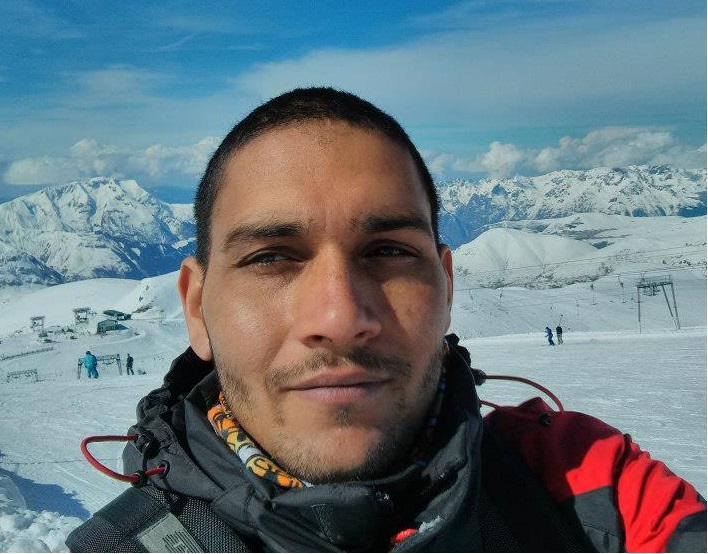
\includegraphics[width=.5\linewidth]{me.jpg}
\end{minipage}
%\noindent
%\parbox{8cm}{}
%\hfill
\section{RESEARCH\\ INTERESTS}
Computer Vision and Machine learning
\section{EDUCATION} 
\textbf{PhD} in Computing and Mathematics   \hfill 15-Sept.-2016 to 30-Sept.-2019 (expected) \\
\textbf{Thesis} topic: \emph{Continuous human action detection and future action prediction.} \\
Supervisors: \href{http://cms.brookes.ac.uk/staff/FabioCuzzolin/}{Dr. Fabio Cuzzolin}\\
\href{http://cct.brookes.ac.uk/research/isec/artificial-intelligence/index.html}{\textbf{Artificial Intelligence and Vision research group}}, Oxford Brookes University\\
Place: Oxford, UK

\textbf{Master of Science in Informatics at Grenoble (MoSIG)}\\
Specialization: \emph{Graphics Vision and Robotics} \hfill 17-September-2012 to 01-July-2013\\
\href{http://ensimag.grenoble-inp.fr/}{\textbf{ENSIMAG - Grenoble INP, France}}\\
Grades: 13.74/20.00  \\
Thesis: \emph{Frame-wise representations of depth videos for action recognition.}\\
Supervisors: Dr. Radu Horaud and Dr. Georgios Evangelidis\\
Place: Grenoble, France
%%Supervisors: \href{https://team.inria.fr/perception/team-members/radu-patrice-horaud/}{Dr. Radu Patrice HORAUD} and \href{https://team.inria.fr/perception/team-members/evangelidis/}{Dr. Georgios EVANGELIDIS}

\textbf{Bacholer of Technology}   \hfill 03-August-2006 to 10-May-2010\\
\textbf{Stream:} Electronics and Instrumentation Engineering\\
\href{http://www.vit.ac.in/}{Vellore Institute of Technology University, Vellore, India};\\
CGPA: 8.33/10.00 \\%%\  \ Max CGPA in class: 9.69/10.00 \\
Thesis: \emph{Categorising the Abnormal Behaviour from an Indoor Overhead Camera.}\\
Supervisor: Dr. Bob Fisher and Dr. P. Arulmozhivaraman\\
Place: Vellore, Tamil Nadu, India

\section{CONTESTS}
ActivityNet, classification and detection challenge (Rank 10/24 and Rank \textbf{2}/6) \hfill 2016\\
Chalearn Looking at People Challenge (Gesture Detection Task Rank 7/17) \hfill 2014\\
Chalearn Multi-Modal Gesture Recognition Challenge (Rank 17/54) \hfill 2013\\

\section{EXPERIENCE}
%\href{http://www.siemens.com/answers/in/en/}
\textbf{Siemens Technology and Services Pvt. Ltd.} \hfill 21-October-2013 to 24-August-15 \\
Research Engineer, Imaging and Computer Vision group\\
Worked on: \emph{Multiple} object detection and tracking for video surveillance applications; 
\emph{Generic} deformable part based models; \emph{Classification} of cancerous lung nodules; \\
Collaborator: Siemens Corporate Research, Princeton, USA \\
Place: Banglore, India

\href{https://team.inria.fr/perception/}{\textbf{Perception team, Inria Grenoble, France}}  \\
Research Engineer: \href{http://gesture.chalearn.org/2013-multi-modal-challenge}{\emph{Multi-modal gesture recognition.}} \hfill 29-July-2013 to 30-Sept-2013 \\
Intern: \emph{Frame-wise representations of depth videos.} \hfill 28-January-2013 to 26-July-2013 \\
Supervisors: Dr. Radu Horaud and Dr. Georgios Evangelidis\\
Place: Grenoble, France

\textbf{\href{http://www.iitd.ac.in/}{Vision and Graphics lab IIT Delhi, India}} \hfill 20-May-2011 to 15-April-2012 \\
Project Associate, \emph{Implementation of Interactive Single View Image Based Model Reconstruction.} AND. 
\emph{Moving object detection with moving camera.} \\
Supervisors: Dr. Subhashis Banerjee\\
Place: New Delhi, India

\textbf{\href{http://www.iitk.ac.in/}{SMSS lab, IIT Kanpur, India}} \hfill 26-July-2010 to 31-March-2011 \\
Project Associate, \emph{Control of Reconfigurable Parabolic Antenna using SMA actuators.}\\
Supervisors: Dr. Bishakh Bhattacharya\\
Place: Kanpur, India

\textbf{\href{http://www.ed.ac.uk/home}{University of Edinburgh, UK} }\hfill 15-January-2010 to 16-May-2010 \\
Undergraduate  Intern: {Institute of Perception, Action and Behaviour} \\ 
Worked on: \emph{Categorising the Abnormal Behaviour from an Indoor Overhead Camera.} \\
Supervisor: Dr. Bob Fisher\\
Place: Edinburgh, UK


\section{PUBLICATIONS}
%\textbf{Gurkirt Singh}, Suman Saha and Fabio Cuzzolin, 
%\emph{Towards real-time action detection and prediction}}, 
%submitted in ACCV 2016, Recived Good reviews, one Strong accept, two weak accept.
Suman Saha, \textbf{Gurkirt Singh}, Michael Sapienza, Philip Torr and Fabio Cuzzolin, 
\emph{Deep Learning for Detecting Multiple Space-Time Action Tubes in Videos}, 
in BMVC 2016, York.

\textbf{Gurkirt Singh} and Fabio Cuzzolin, 
\emph{Untrimmed Video Classification for Activity Detection: submission to ActivityNet Challenge}, 
arXiv preprint arXiv:1607.01979 (2016), \textbf{2nd} position in Activity Detection challenge at ActivityNet workshop CVPR 2016.

Georgios Evangelidis, \textbf{Gurkirt Singh}, Radu Horaud, 
%\href{https://sites.google.com/site/gurkirtcv/research/continuous}
{\emph{Continuous Gesture Recognition from Articulated Poses}}, 
in ChalearnLAP2014 workshop at EECV  2014, Zurich. \textbf{17} citations

%This work was carried out in context of in Multi-modal gesture recognition challenge 2014. Our team ranked 8th out of 17 by using only Skeleton information.\\
%Keywords: gesture detection, dynamic programming, skeleton descriptor
Georgios Evangelidis, \textbf{Gurkirt Singh}, Radu Horaud,
\href{https://team.inria.fr/perception/research/icpr2014/}{\emph{Skeletal Quads: Human action recognition using joint quadruples}}, 
in ICPR 2014 Stockholm. \textbf{44} citations
%We propose a local skeleton descriptor that encodes the relative position of joint quadruples. Such a coding implies a similarity normalisation transform that leads to a compact (6D) view-invariant skeletal feature. 
%Further, the use of a Fisher kernel representation is suggested to describe the skeletal quads contained in a action. \\
%Keywords: multi-level Fisher vectors, linear SVM
\section{THESIS}
%\textbf{Gurkirt Singh} and Georgios Evangelidis, {\emph{Participated in Multi-modal gesture recognition 2013 using RGB-D, Skeleton and Audio}}, 
%\href{http://gesture.chalearn.org/2013-multi-modal-challenge}
%11th out of 17 by using alone Skeleton information.
%We build a BOW representation of using skeleton-quad  descriptors from human joint positions. Dynamic programming was used for simultaneous recognition and segmentation of gestures. \\

\textbf{Master's thesis}, \href{https://sites.google.com/site/gurkirtcv/research/master-thesis}{\emph{Frame-wise Representations of Depth Videos for Action Recognition.}}\\
We investigate the of problem continuous action recognition from depth images. 
Three types of depth frame data representation are proposed. 
Further, we investigate the frame-wise classification as a solution for the continuous action detection problem.

\textbf{Bachelor's thesis} \href{https://sites.google.com/site/gurkirtcv/research/btechproject}{\emph{Categorising the Abnormal Behaviour from an Indoor Overhead Camera.}}
We propose an approach using an overhead camera to detect the moving objects (Persons). A tracker is used to track their trajectories. 
Spline fitting is used to represent the trajectories with equal number of attributes. 
Finally abnormal trajectories are detected with Gaussian mixture model based classification. 
The system detects the anomalous events with EER (Equal Error rate) of only 1.2\%. 
Contribution of 65000 pedestrian trajectories to \href{http://homepages.inf.ed.ac.uk/rbf/FORUMTRACKING/}{\emph{“Edinburgh Informatics Forum Pedestrian Database”}}.

\section{SKILLS}
\textbf{Programming Languages:} Python, Matlab, C/C++.\\
\textbf{Libraries:} OpenCV, Eigen, Scikit-Learn, Numpy, Scipy, Theano, Caffe, Kinect SDK\\
\textbf{Operating Systems:} Linux and Windows.\\
\textbf{Development Environments:} Visual Studio, Eclipse, GCC, Spyder.\\


\section{MISC}
Attended International Computer Vision  Summer school 2016. Sicili, part of winning reading group.
%\section{LANGUAGES}
%Punjabi (Maternal), Hindi (Fluent), English (Fluent), French (Elementary)
\end{resume}
\end{document}
